\documentclass[11pt]{article}
\usepackage[T1]{fontenc}
\usepackage[margin=0.85in]{geometry}
\usepackage{graphicx}
\usepackage{xcolor}
\usepackage{listings}
\usepackage{booktabs}
\usepackage{hyperref}
\definecolor{codeblue}{RGB}{36,83,150}
\definecolor{codestring}{RGB}{145,50,45}
\definecolor{codegreen}{RGB}{45,115,75}
\definecolor{codegray}{RGB}{100,100,100}
\lstdefinestyle{python}{
  language=Python, basicstyle=\ttfamily\small,
  keywordstyle=\color{codeblue}\bfseries, stringstyle=\color{codestring},
  commentstyle=\color{codegreen}\itshape, numberstyle=\scriptsize\color{codegray},
  numbers=left, numbersep=8pt, showstringspaces=false, breaklines=true,
  frame=single, rulecolor=\color{black!20}, columns=fullflexible,
  keepspaces=true, upquote=true, tabsize=4
}
\lstset{style=python}
\hypersetup{colorlinks=true,linkcolor=blue!50!black,urlcolor=blue!50!black}
\title{Early Bearish News in a Bubble-Prone Asset Market\\\large EDSL shared-state pilot}
\author{EDSL replication study}
\date{October 11, 2026}

\begin{document}
\maketitle

\begin{abstract}
Six of twelve traders received a private downside analyst forecast before the
first order in a 30-period call market. The remaining market rules and the
behavioral instructions matched a separate bullish-news pilot: four momentum
buyers, four bubble riders, and four profit-taking sellers. The bearish update
did not prevent an early rise. Prices increased from \$15.25 to \$20.00 by
period 10 and reached \$26.50 in period 29; 51 shares traded across 22 periods.
Treated and untreated price forecasts converged quickly. First-period rationales
show that traders often prioritized their assigned behavior over the private
downside signal. The result is one exploratory market session, not an estimate
of a causal news effect.
\end{abstract}

\section{Market and intervention}
The market has 12 traders, each starting with \$100 cash and four shares. Cash
earns 5\% interest; each share pays \$0.40 or \$1.00 with equal probability;
remaining shares are redeemed for \$14 after period 30. The deterministic
uniform-price call market uses the same settlement and payoff rules as the
bullish bubble pilot.

All traders receive one of three behavioral instructions: four momentum buyers,
four bubble riders, or four profit-taking sellers. The instructions provide
opening order anchors to make two-sided trade more likely. Two participants
from each behavior group are assigned to receive the private update. Before
period 1, the report says expected resale demand has weakened and prices could
fall toward \$10 by period 10. The update clearly says this is an uncertain
forecast and that dividends and the actual \$14 redemption are unchanged.
Recipients: trader-00 and trader-01 (momentum), trader-05 and trader-07 (bubble
riders), trader-08 and trader-10 (profit takers).

\section{Observed results}
\begin{center}
\begin{tabular}{lr}
\toprule
Measure & Pilot result \\
\midrule
Trader decisions & 360 \\
Settlements & 30 / 30 \\
Private update deliveries & 6 \\
Completed workflow items & 396 / 396 \\
Shares traded & 51 \\
Periods with trade & 22 / 30 \\
Peak transaction price & \$26.50 \\
Terminal shares & 0 for every trader \\
Terminal cash range & \$538.65--\$799.35 \\
\bottomrule
\end{tabular}
\end{center}

Transactions occurred in periods 1--4, 6--10, 14--25, and 29. The price was
\$15.25 in period 1, rose to \$20.00 in period 10, and continued to \$26.50 in
period 29. It exceeded the \$14 terminal redemption value throughout observed
transactions. The news forecast of a possible fall toward \$10 was not realized
in this market path.

Across 360 decisions, traders submitted 171 buy orders, 99 sell orders, and 90
holds. Momentum traders submitted 116 buys. Bubble riders submitted 40 buys and
76 sells, consistent with building positions and then offering shares. The
profit-taker group chose hold 86 times, sell 19 times, and buy 15 times.

In period 1, update recipients' mean current-price forecast was \$14.50, versus
\$15.00 for the no-news group. By period 10, means were \$19.67 and \$19.75;
by period 25 they were \$25.83 and \$26.00. Treated momentum traders explicitly
said they would buy early despite the update; treated bubble riders emphasized
speculative demand; treated profit takers cited the update as a reason to sell.
These are descriptive responses from six traders per group in a single shared
market.

\begin{figure}[ht]
\centering
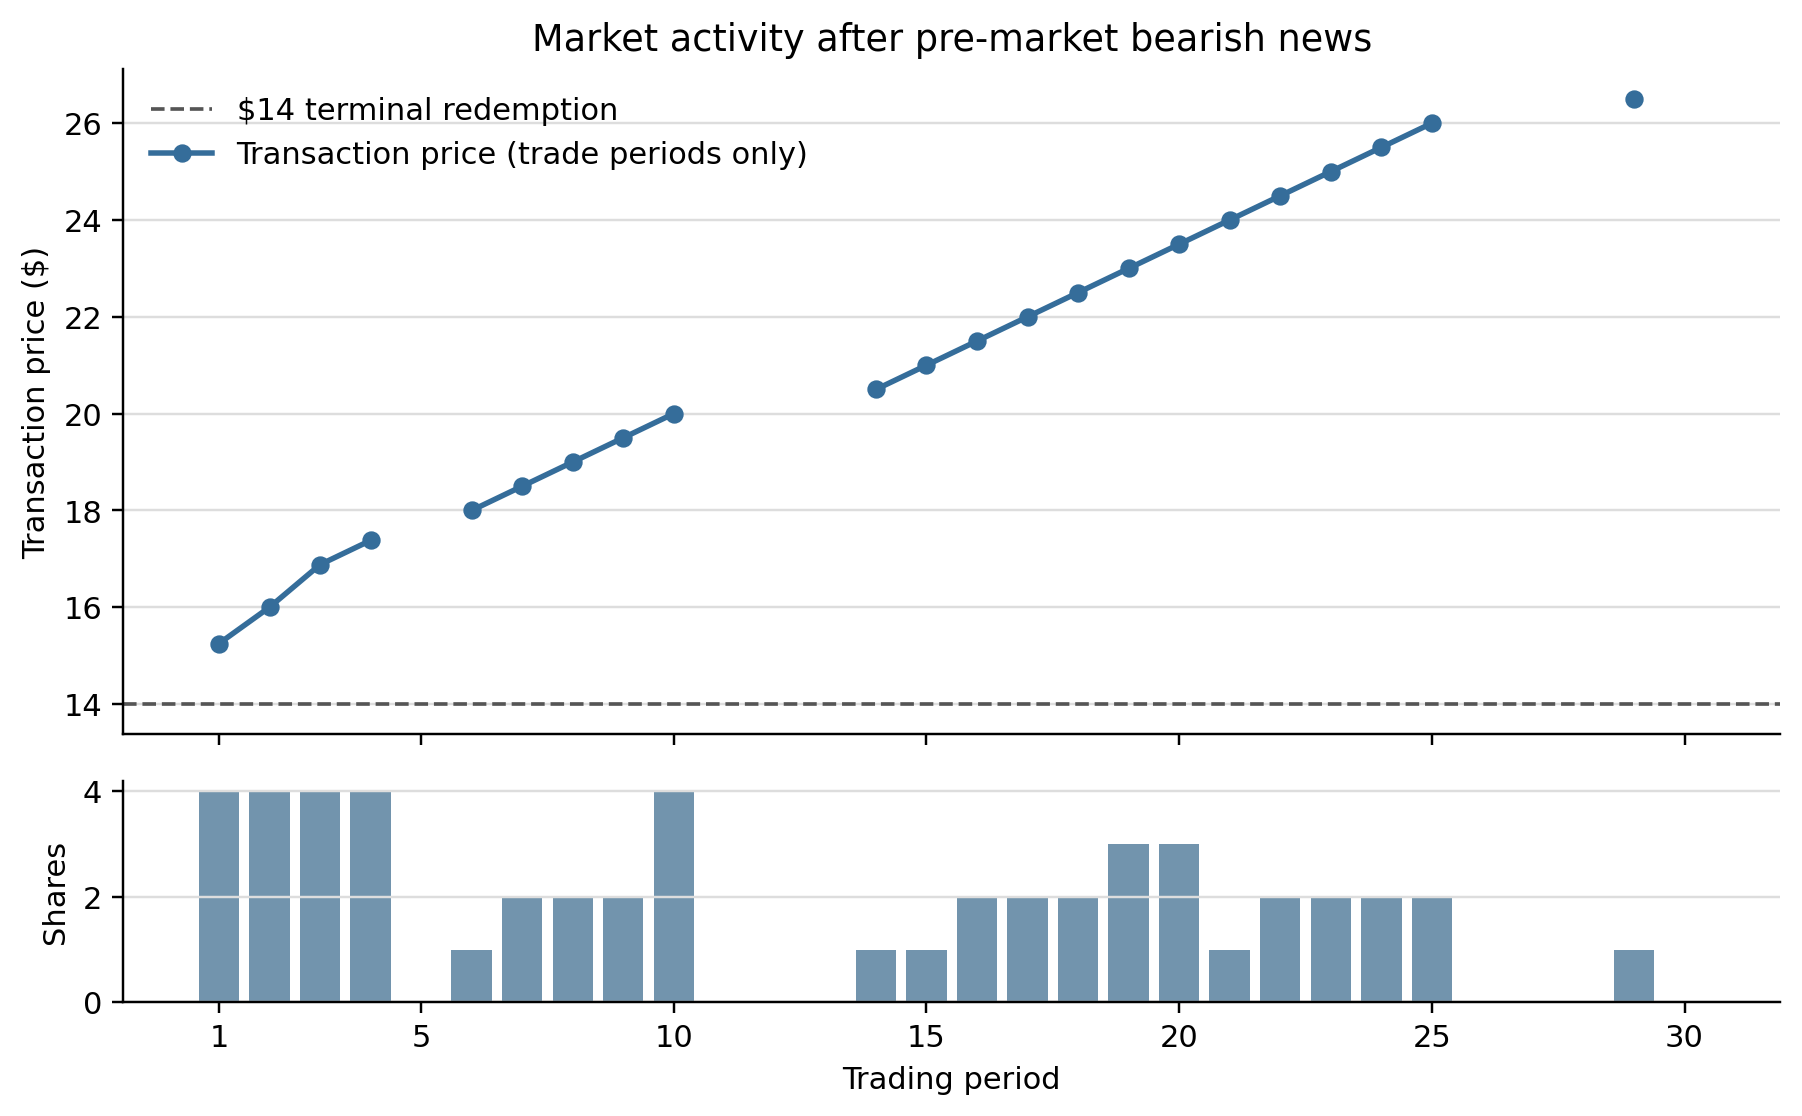
\includegraphics[width=0.88\linewidth]{market_outcomes.png}
\caption{Transaction prices and traded volume. The dashed line marks the \$14
terminal redemption amount. Missing prices indicate no transaction.}
\end{figure}

\begin{figure}[ht]
\centering
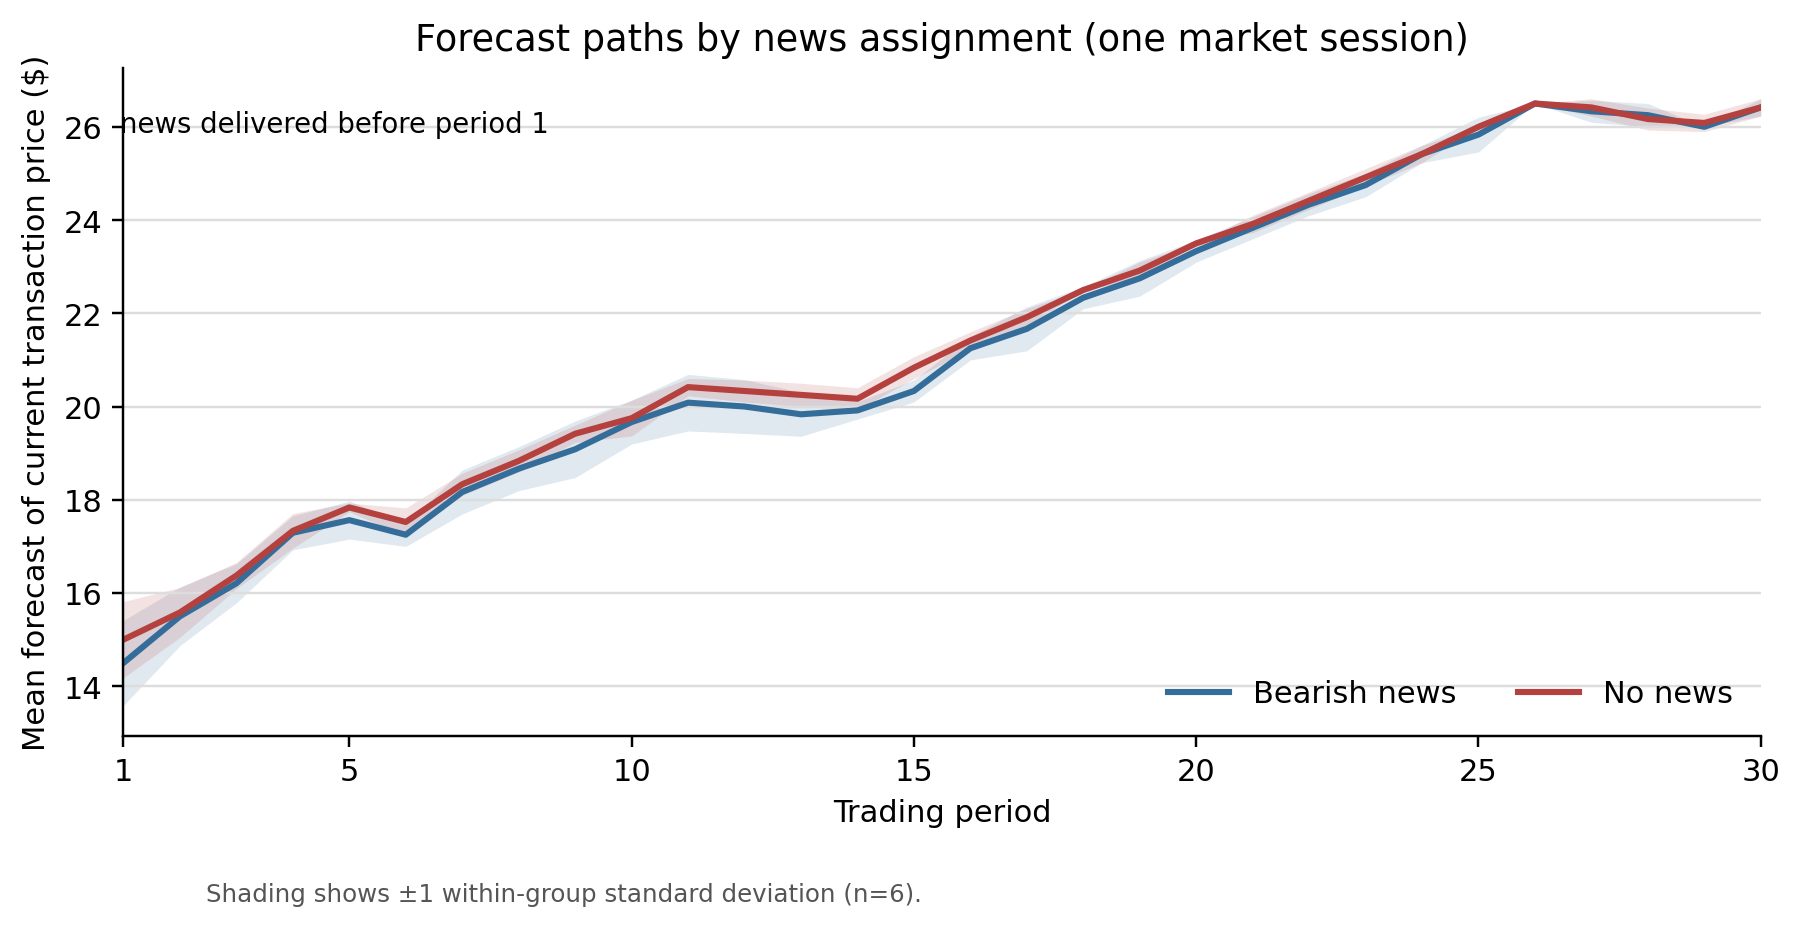
\includegraphics[width=0.88\linewidth]{forecast_paths.png}
\caption{Mean current-price forecasts by news assignment. Shading shows one
within-group standard deviation ($n=6$), not a confidence interval. The update
was delivered before period 1.}
\end{figure}

Relative to the separate bullish-news pilot, this run traded 51 rather than 22
shares and reached \$26.50 rather than \$18.00. Since each comparison is a
single independently run market, differences cannot be attributed to news
direction or timing. The pattern is consistent with behavior prompts and market
feedback overwhelming a private downside forecast, but repeated markets are
needed to test that interpretation.

\section{Shared-state machine}
The experiment extends EDSL's native \texttt{call\_market} machine with a map
that stores private messages, a command to publish a message, and a participant
view that selects the entry for the current trader. The map is omitted from the
trader-facing view; each participant receives only their own update.

\begin{lstlisting}
machine = call_market(TRADERS, rules=RULES, seed=SEED)
machine.fields["private_updates"] = state_field(StateType.map(), {})
machine.commands["publish_update"] = Command(
    inputs={"recipient": StateType.text(), "message": StateType.text()},
    effects=(put("private_updates", arg("recipient"), arg("message")),),
)
machine.view["your_update"] = field("private_updates").get(current("name"))
machine.validate()
\end{lstlisting}

Each write is an exchange task assigned to the scripted executor. Six such
tasks are placed before period 1. The first trader order step depends on all
six, which guarantees the state write completes before the initial decision.
The view expression returns an empty value to traders absent from the private
map.

\begin{lstlisting}
for recipient in recipients:
    publish_steps.append(workflow.step(
        f"publish-private-update-{recipient}", update_survey,
        assigned_to=role("exchange"),
        writes=(market.publish_update(
            recipient=recipient, message=UPDATE,
        ),),
    ))
previous = publish_steps
for period in range(1, PERIODS + 1):
    orders = workflow.step(
        f"orders-{period}", Survey([decision]),
        assigned_to=role("trader"), after=previous,
        reads=(market.read(),),
        writes=(market.submit(
            trader=current.agent.name, period=period,
            decision=decision.answer,
        ),),
    )
    settled = workflow.step(
        f"settle-{period}", settlement_survey,
        assigned_to=role("exchange"), after=orders,
        writes=(market.settle(period=period),),
    )
    previous = settled
\end{lstlisting}

The first period therefore begins after information publication; later periods
retain the ordinary order-then-settlement chain. The six information tasks do
not call a model. The detailed machine diagram was generated by EDSL's native
\texttt{Machine.show\_diagram} method.

\begin{figure}[ht]
\centering
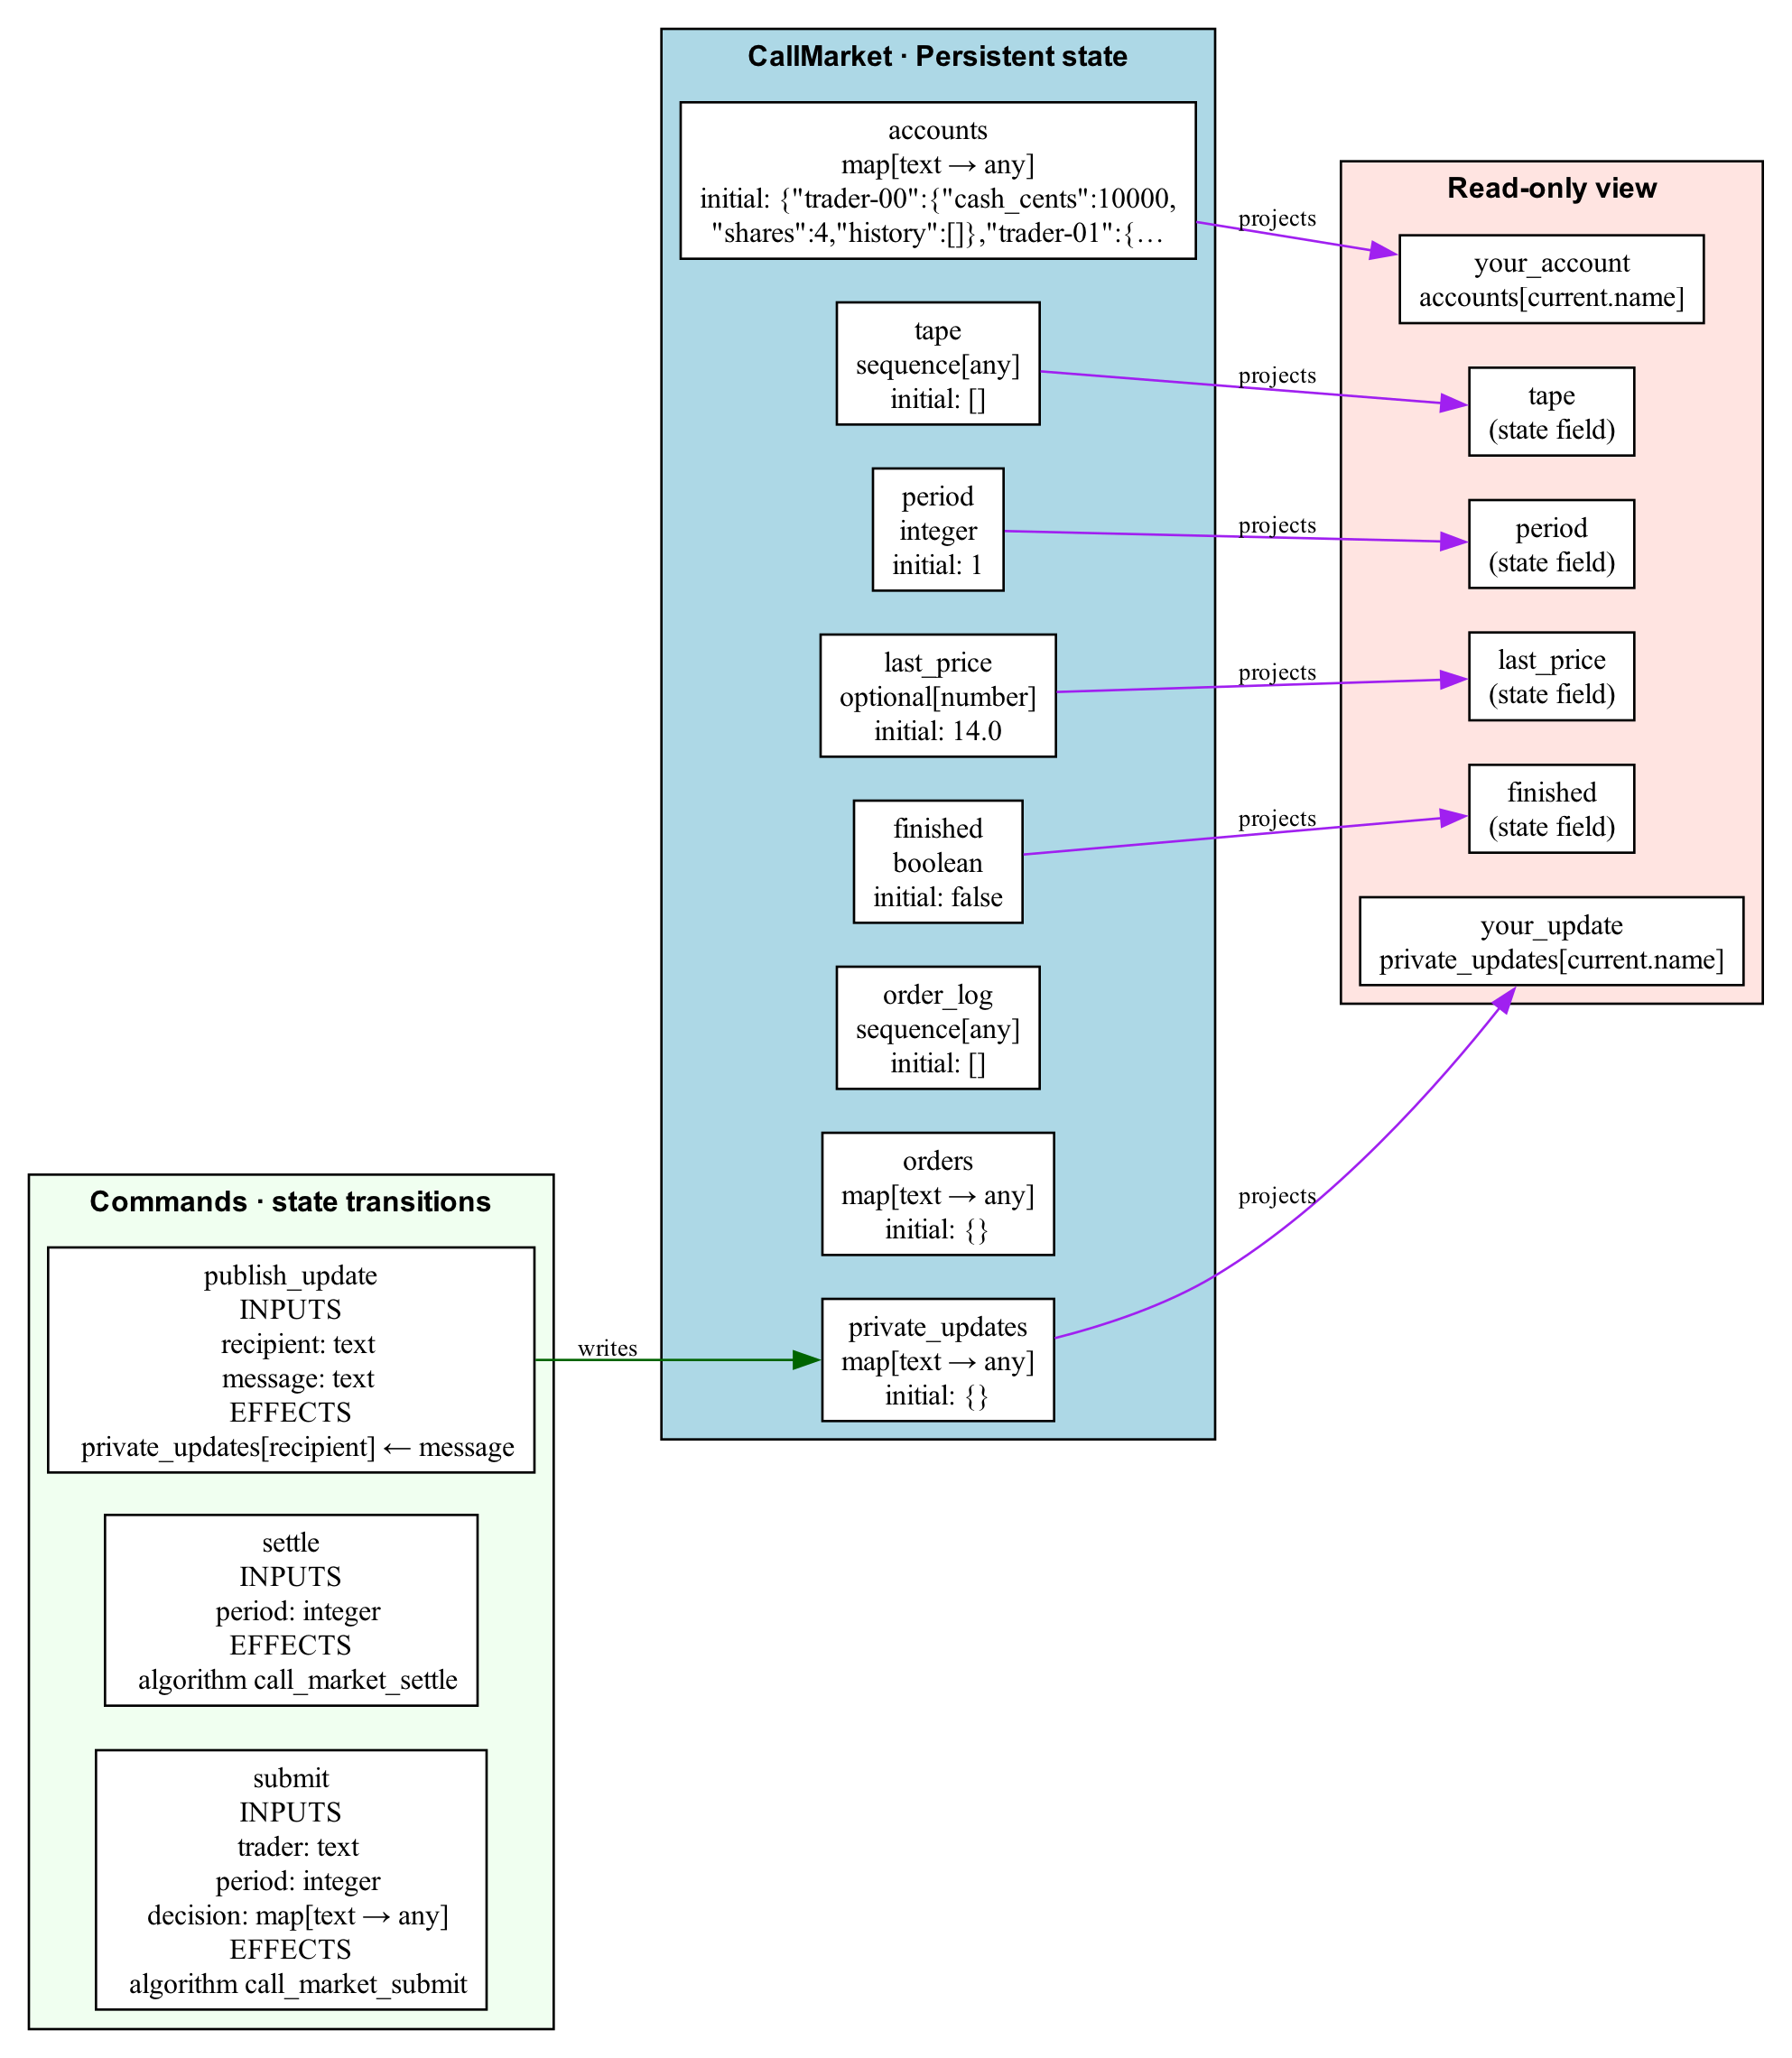
\includegraphics[width=0.62\linewidth,height=0.70\textheight,keepaspectratio]{market_machine.png}
\caption{Detailed call-market machine with the private update field and command.}
\end{figure}

\section{Run and limits}
The experiment was run locally through EDSL with the configured provider
credentials. The workflow, jobs, model calls, shared-state SQLite log, and
completion record are preserved in \texttt{pilot\_01/}. The standalone
specification can be rebuilt without model calls using:

\begin{lstlisting}
python3 edsl_replication/studies/asset_market_bearish_early/experiment.py \\
  --output edsl_replication/studies/asset_market_bearish_early/pilot_01 \\
  --prepare-only
\end{lstlisting}

This one market has a mixed treatment and one shared public tape, so traders
affect one another. A factorial design should vary news sign, delivery time,
and behavioral prompts independently over repeated seeds. That would separate
the effect of bearish information from assigned speculative behavior and
endogenous price feedback.

\end{document}
